%\documentclass[aspectratio=169]{beamer}
\documentclass{beamer}
\usetheme{PaloAlto}
%\usetheme{AnnArbor}
\setbeamercovered{transparent}

\usepackage[utf8]{inputenc}

\title{Curso de BEAMER.}
\author[Felipe]{Felipe F. Soares.}
\institute[UFC]{Universidade Federal do Ceará \\ ufc.br}
\date{2016}
%\date{}
%\date{Nome do evento, 2016}
\logo{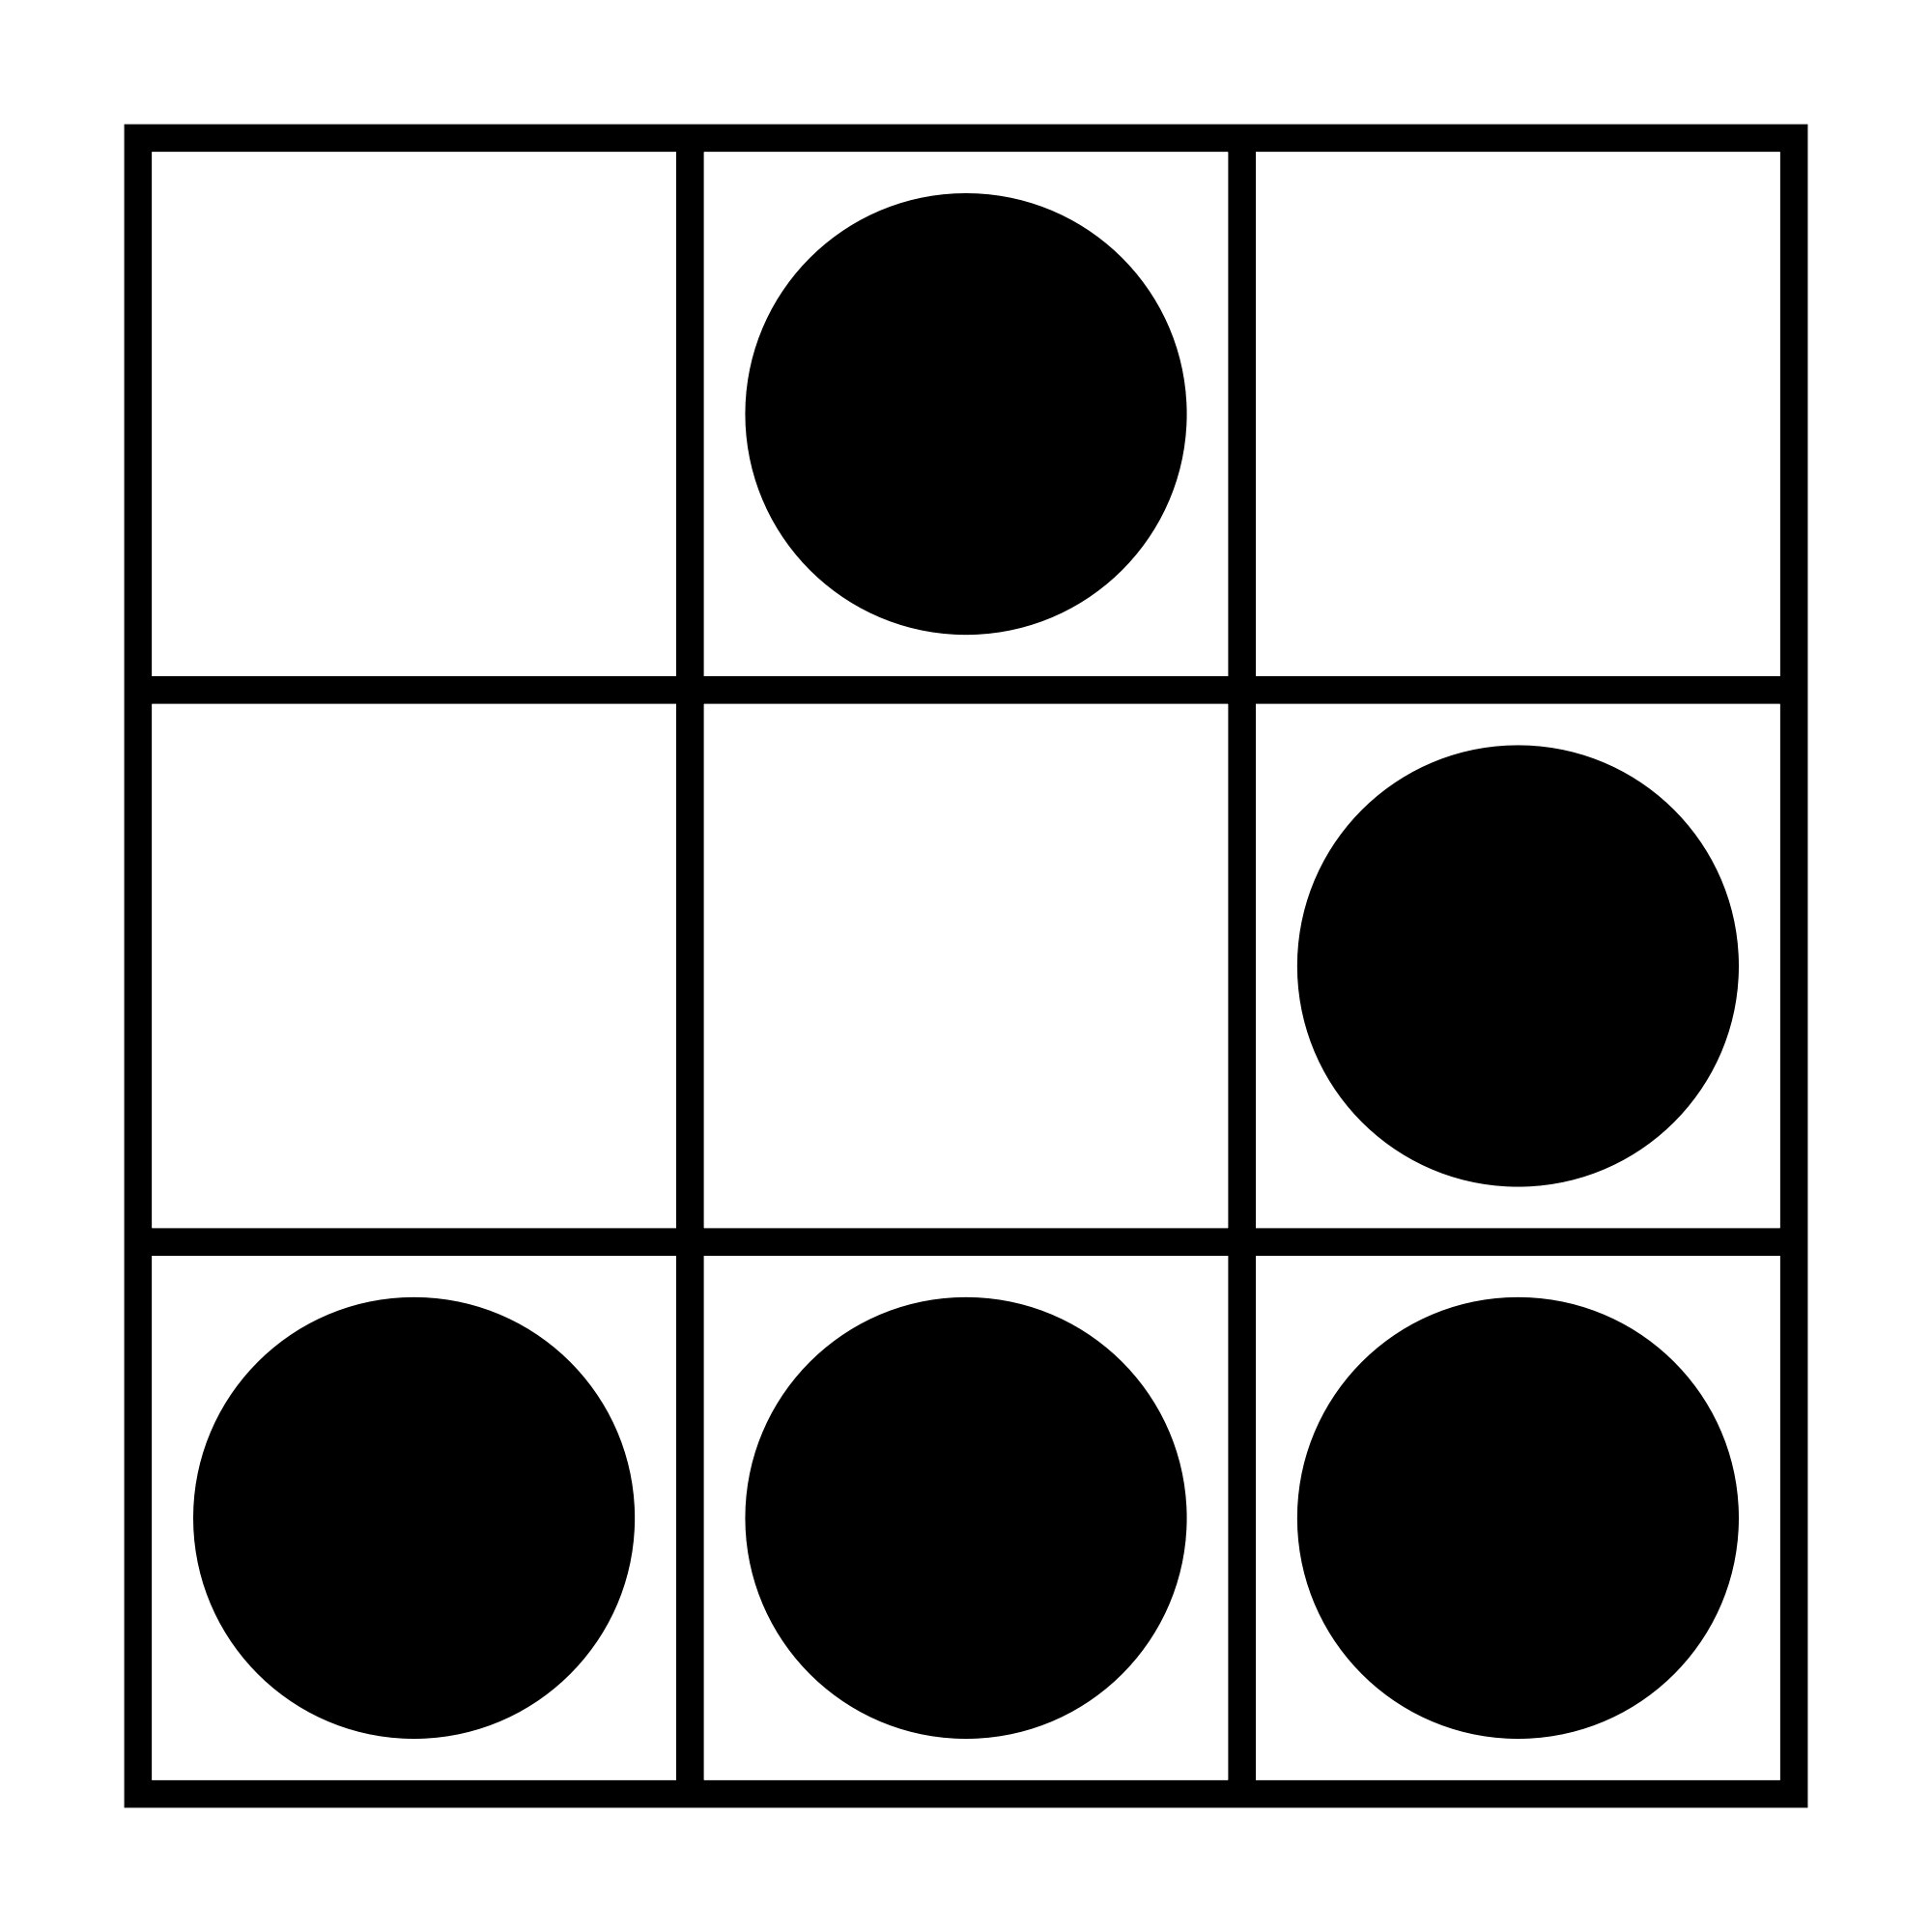
\includegraphics[scale=0.01]{images/glider.png}}

\AtBeginSection[]{
	\begin{frame}
	%\tableofcontents
	%\tableofcontents[currentsection,]
	%\tableofcontents[currentsection, hideallsubsections]
	\tableofcontents[currentsection, hideothersubsections]
	\end{frame}
}

\AtBeginSubsection[]{
	\begin{frame}
	%\tableofcontents
	\tableofcontents[currentsubsection]
	\end{frame}
}

\begin{document}
	\begin{frame}{Esse é o título do quadro}
		\titlepage
	\end{frame}
	
	\begin{frame}
		\frametitle{Sumário}
		%\tableofcontents
		\tableofcontents[part=1]
	\end{frame}
	
	\begin{frame}
		\frametitle{Sumário}
		%\tableofcontents
		\tableofcontents[part=2]
	\end{frame}
	
	\begin{frame}{Esse é o título do quadro}
		\frametitle{Sumário}
		%\tableofcontents
		\tableofcontents[pausesections, pausesubsections]
	\end{frame}
	
	\part{Revisão}
	\section[Introdução]{Uma Introdução com título grande}
	\begin{frame}{Esse é o título do quadro}
		\frametitle{Aqui é o título}
		\framesubtitle{Aqui é o subtitulo}
		Esse é o quadro 1
	\end{frame}
	
	\section{Metodologia}
	\subsection{Uma subseção da metodologia}
	\begin{frame}{Esse é o título do quadro}
		\frametitle{Aqui é o título}
		\framesubtitle{Aqui é o subtitulo}
		Esse é o quadro 2 %\cite{meuartigo}
	\end{frame}
	
	\subsection{Uma outra subseção da metodologia}
	\begin{frame}{Esse é o título do quadro}
		\frametitle{Aqui é o título}
		\framesubtitle{Aqui é o subtitulo}
		Esse é o quadro 3
	\end{frame}
	
	\section{Discussão}
	\subsection{Uma subseção da discussão}
	\begin{frame}{Esse é o título do quadro}
		\frametitle{Aqui é o título}
		\framesubtitle{Aqui é o subtitulo}
		Esse é o quadro 4 %\cite{meuartigo}
	\end{frame}
	
	\begin{frame}{Esse é o título do quadro}
		\frametitle{Aqui é o título}
		\framesubtitle{Aqui é o subtitulo}
		Esse é o quadro 5
	\end{frame}
	
	\subsection{Uma outra subseção da discussão}
	\begin{frame}{Esse é o título do quadro}
		\frametitle{Aqui é o título}
		\framesubtitle{Aqui é o subtitulo}
		Esse é o quadro 6
	\end{frame}
	
	\subsection{Uma outra subsubseção da discussão}
	\begin{frame}{Esse é o título do quadro}
		\frametitle{Aqui é o título}
		\framesubtitle{Aqui é o subtitulo}
		Esse é o quadro 6.1
	\end{frame}
	
	\section{Conclusão}
	\begin{frame}{Esse é o título do quadro}
		\frametitle{Aqui é o título}
		\framesubtitle{Aqui é o subtitulo}
		Esse é o quadro 7
	\end{frame}
	
	\begin{frame}{Esse é o título do quadro}
		\frametitle{Aqui é o título}
		\framesubtitle{Aqui é o subtitulo}
		Esse é o quadro 8
	\end{frame}
	
	%\section*{Referências}
	%\begin{frame}
		%\bibliographystyle{plain}
		%\bibliographystyle{apalike}
		%\bibliography{•}
	%\end{frame}
	
	
	\part{Aula de hoje}
	\section[Introdução]{Uma Introdução com título grande}
	\begin{frame}{Esse é o título do quadro}
		\frametitle{Aqui é o título}
		\framesubtitle{Aqui é o subtitulo}
		Esse é o quadro 1
	\end{frame}
	
	\section{Metodologia}
	\subsection{Uma subseção da metodologia}
	\begin{frame}{Esse é o título do quadro}
		\frametitle{Aqui é o título}
		\framesubtitle{Aqui é o subtitulo}
		Esse é o quadro 2 %\cite{meuartigo}
	\end{frame}
	
	\subsection{Uma outra subseção da metodologia}
	\begin{frame}{Esse é o título do quadro}
		\frametitle{Aqui é o título}
		\framesubtitle{Aqui é o subtitulo}
		Esse é o quadro 3
	\end{frame}
	
	\section{Discussão}
	\subsection{Uma subseção da discussão}
	\begin{frame}{Esse é o título do quadro}
		\frametitle{Aqui é o título}
		\framesubtitle{Aqui é o subtitulo}
		Esse é o quadro 4 %\cite{meuartigo}
	\end{frame}
	
	\begin{frame}{Esse é o título do quadro}
		\frametitle{Aqui é o título}
		\framesubtitle{Aqui é o subtitulo}
		Esse é o quadro 5
	\end{frame}
	
	\subsection{Uma outra subseção da discussão}
	\begin{frame}{Esse é o título do quadro}
		\frametitle{Aqui é o título}
		\framesubtitle{Aqui é o subtitulo}
		Esse é o quadro 6
	\end{frame}
	
	\subsection{Uma outra subsubseção da discussão}
	\begin{frame}{Esse é o título do quadro}
		\frametitle{Aqui é o título}
		\framesubtitle{Aqui é o subtitulo}
		Esse é o quadro 6.1
	\end{frame}
	
	\section{Conclusão}
	\begin{frame}{Esse é o título do quadro}
		\frametitle{Aqui é o título}
		\framesubtitle{Aqui é o subtitulo}
		Esse é o quadro 7
	\end{frame}
	
	\begin{frame}{Esse é o título do quadro}
		\frametitle{Aqui é o título}
		\framesubtitle{Aqui é o subtitulo}
		Esse é o quadro 8
	\end{frame}
	
	%\section*{Referências}
	%\begin{frame}
		%\bibliographystyle{plain}
		%\bibliographystyle{apalike}
		%\bibliography{•}
	%\end{frame}
	
\end{document}